\documentclass[uplatex]{jsarticle}
\usepackage[dvipdfmx]{graphicx}
\title{ソフトウェア設計法2}

\author{101730153 佐治 礼仁 saji.ayahito@h.mbox.nagoya-u.ac.jp}
\date{\today}
\begin{document}
\maketitle
\section{自身でシステムで実装する簡単な情報の流れを定義せよ}
題材として,Compassのような「イベント申し込みプラットフォーム」を用いることにする.
次のような仕様とする.

まず企画者は,企画の情報をシステムに登録を行う.ここで企画の情報とは,日時,イベント名,参加人数上限,参加費用である.
参加者は,参加したいイベントを選び,参加依頼を行う.参加するために,氏名,年齢,メールアドレスを必要とする.
イベントに参加できるようであれば,参加者のメールアドレスに参加可能である旨のメールが届く.

\section{コンテキスト図とデータフロー図}
コンテキスト図を図\ref{fig:context-diagram},データフロー図を図\ref{fig:dataflow-diagram}に示す.

\begin{figure}[htbp]
  \begin{center}
    
\includegraphics[clip,width=10.0cm]{figures/context-diagram.png}
    \caption{コンテキスト図}
    \label{fig:context-diagram}
  \end{center}
\end{figure}


\begin{figure}[htbp]
  \begin{center}
    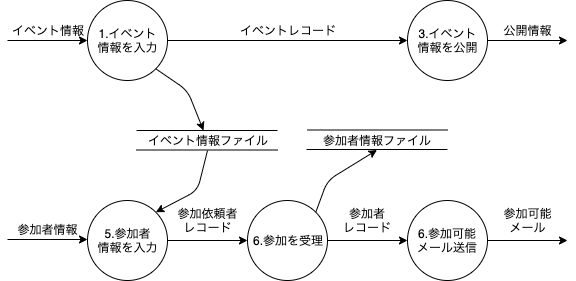
\includegraphics[clip,width=10.0cm]{figures/dataflow-diagram.png}
    \caption{データフロー図}
    \label{fig:dataflow-diagram}
  \end{center}
\end{figure}


\end{document}
